\section{Main elements and workflow}

Each Lambert's problem solver makes use of its own mathematical background to
find the solution to the problem. However, all algorithms share a common
workflow in which a particular set of elements can be identified. Among these
elements it is possible to find the free-parameter, the numerical method, an
initial-guess and the velocity vectors construction procedure.

\vspace{0.5cm}
\begin{figure}[h]
  \centering
  \includegraphics[width=\linewidth]{static/solver_workflow.pdf}
  \caption{Main elements forming the basic structure of any modern Lambert's
    problem solver.}
  \label{fig:solver_elements}
\end{figure}

It must be pointed out that some methods developed along history, which will be
presented in future pages, solve the Lambert's problem by making use of a series
expansion. Therefore, the accuracy of the method is based on the number of
terms considered instead of requiring a numerical method. However, apart from
these type of solvers, the rest of them share the elements presented in figure
\ref{fig:solver_elements}.

\subsection{The free-parameter}

The free-parameter is the independent variable, also named the iteration
variable. This variable appears in an implicit way in a fundamental equation of
the algorithm, meaning that a numerical method is required in order to solve for
it. Once its value has been computed, each algorithm will follow a particular
approach to solve for the rest of the orbital elements.

Among history, several algorithms have been developed exploiting different
free-parameters such us the semi-major axis $a$, the orbit's eccentricity $e$,
the orbital parameter or semi-latus rectum $p$, the true anomaly $\nu$, the
universal formulation and finally the Kustaanheimo-Stiefel formulation and the
flight path angle $\gamma$.

\vspace{0.5cm}
\begin{figure}[h]
  \centering
  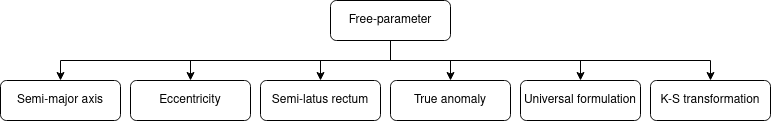
\includegraphics[width=\linewidth]{static/free_parameter.pdf}
  \caption{All possible free-parameters employed for solving the Lambert's problem.}
  \label{fig:free_parameter}
\end{figure}

\subsection{The initial guess}

Before the iterative process can start, an initial guess is required. This is
the starting value imposed to the free-parameter, so the closer it is to the
solution, the lower the amount of iterations till the free-parameter converges
to a desired accuracy.

Classic algorithms, all of those previous to the modern ones, made use of an
arbitrary initial guess without developing any additional procedure. This is no
longer the case with modern ones in which a more complex sub-routine is provided
in order to have a reliable initial guess to reduce the computation time and
faster achieve the solution.

The initial guess is dependent on the numerical method employed and thus, on the
mathematical background too. A total of three common solutions have been
identified in literature, being these the rational formulate, linear approach
and bi-linear one, as depicted by diagram in figure \ref{fig:initial_guess}.

\vspace{0.5cm}
\begin{figure}[h]
  \centering
  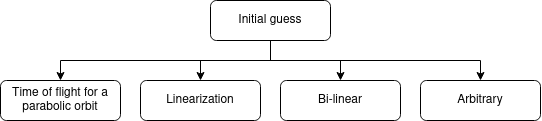
\includegraphics[scale=0.80]{static/initial_guess.pdf}
  \caption{Possible approaches to be used in the initial guess procedure.}
  \label{fig:initial_guess}
\end{figure}

The rational formulate (also named arbitrary initial guess) is based on the time
of flight curves against the free-parameter. By identifying different regions
and their expected time of flight it is possible to compare those against the
current one and estimate the solution.

Regarding the linear approach and bi-linear guesses, these simplify the
free-parameter transcendental equation so that it becomes an explicit one.
Although very useful, not all the equations for the free-parameter might be
benefit from this initial guess.

It must be pointed that the level of complexity of initial guess procedure must
not be detrimental from the point of view of the total computation time.
Otherwise, it is absurd to waste such a valuable time instead of letting the
root solver to perform the iteration workload.

\subsection{The numerical method}

The previously presented free-parameter is solved by means of a numerical method
or root finder. Numerical methods for solving root equations are abundant in the
literature, being some of the most common ones bisection, regula falsi, secant,
Newton's method, Halley's method and Householder's one\footnote{Notice that
  Newton's and Halley's methods are just Householder's one but of lower order.}.

\vspace{0.5cm}
\begin{figure}[h]
  \centering
  \includegraphics[width=\linewidth]{static/root_solver.pdf}
  \caption{Different root finders found in literature to solve for the
    free-parameter equation.}
  \label{fig:numerical_method}
\end{figure}


The last three of the listed methods are the most common ones employed by
authors in modern solvers. However, these methods required from the derivative
of the free-parameter transcendental equation with respect to the free-parameter
itself. Equations \ref{eq:newtons_method}, \ref{eq:halleys_method} and
\ref{eq:householders_method} present these three methods where $x_n$ and
$x_(n+1)$ inditcate the current and next free-parameter value, $f$ is the
function to be evaluated and $f'$, $f''$ its first and second derivatives.

\begin{align}
  \text{Newton's method} \quad\quad      & x_{n+1} = x_{n} - \frac{f(x_n)}{f'(x_n)} \label{eq:newtons_method}                                                                       \\
  \text{Halley's method} \quad\quad      & x_{n+1} = x_{n} - \frac{2f(x_n)f'(x_n)}{2\left[f'(x_n)\right]^{2} - f(x_n)f''(x_n)} \label{eq:halleys_method}                            \\
  \text{Householder's method} \quad\quad & x_{n+1} = x_{n} - \frac{f(x_n)}{f'(x_n)}\left(1 + \frac{f(x_n)f''(x_n)}{2\left[f'(x_n)\right]^{2}}\right) \label{eq:householders_method}
\end{align}


Previous methods are preferred due to its performance and accuracy. However, not
all the transcendental equations have a simple derivative. In most of the cases
this one becomes quite complex and authors end up using the secant method. Not
only that, previous methods are singular for values of $x_n$ such that
$f'(x_n)=0$.

When previous situation applies, some authors impose a change in the root solver
so that bisection or regula-falsi methods are used. These two methods, once the
solution has been bounded, guarantee the convergence to the right value of the
free-parameter. However, they rate of converge is slower if compared against
Newton's, Halley's or Householder's method.

\subsection{The velocity vectors construction}

The last sub-routine employed by any Lambert's solver is the computation of the
velocity vectors. One might thought that the computation of COE elements is also
valid but, since we are given as initial input two position vectors, it is
reasonable that the user expects the velocity vectors as output so the RV set is
completely defined.

There are different approaches followed by modern solvers to compute the value
of these vectors once the free-parameter has been solved such us using the
radial and tangential components, $f$ and $g$ formulation\footnote{This is also
  known as Gauss' $f$ and $g$ formulae.} introduced in \cite{bate1971} or applying a
COE to RV conversion.

\vspace{0.5cm}
\begin{figure}[h]
  \centering
  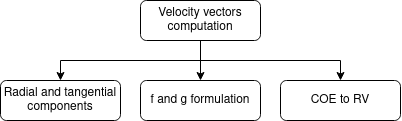
\includegraphics[scale=0.80]{static/velocity_vectors.pdf}
  \caption{Possible ways of constructing the initial and final velocity vectors.}
  \label{fig:velocity_vectors}
\end{figure}

The radial and tangential components can computed from equation
\ref{eq:radia_tangential_v}, where $h_0$ is obtained via previously presented
\ref{eq:normal_vector} and the values of $v_{r_1}$, $v_{r_2}$, $v_{t_1}$ and
$v_{t_1}$ computed using a particular solver.

\begin{equation}
  \vec{v_{1}} = v_{r_1} \frac{\vec{r_1}}{\norm{\vec{r_1}}} + v_{t_1} \frac{\vec{h_0} \times \vec{r_1}}{\norm{\vec{h_0} \times \vec{r_1}}}\quad\quad\quad
  \vec{v_{2}} = v_{r_2} \frac{\vec{r_2}}{\norm{\vec{r_2}}} + v_{t_2} \frac{\vec{h_0} \times \vec{r_2}}{\norm{\vec{h_0} \times \vec{r_2}}}
  \label{eq:radia_tangential_v}
\end{equation}

Another common way of computing the velocity vectors at the initial and final
points is to use the $f$ and $g$ formulation, see \ref{eq:f_and_g_v}:

\begin{equation}
  \vec{v_1} = (\vec{r_2} - f \vec{r_1}) / g \quad\quad\quad
  \vec{v_2} = (\dot{g} \vec{r_2} - \vec{r_1}) / g
  \label{eq:f_and_g_v}
\end{equation}

where the values for the $f$, $g$, $\dot{f}$ and $\dot{g}$ can be obtained using
the following relations:

\begin{align}
  f       & = 1 - \frac{a}{\norm{\vec{r_1}}} \left(1 - \cos{(\Delta E)} \right)          \\
  g       & = \Delta t - \sqrt{\frac{a^3}{\mu}} \left(\Delta E - \sin{(\Delta E)}\right) \\
  \dot{f} & = \frac{-\sqrt{\mu a}}{\norm{\vec{r_1}} \norm{\vec{r_2}}}                    \\
  \dot{g} & = 1 - \frac{a}{\norm{\vec{r_2}}} \left(1 - \cos{(\Delta E)} \right)
\end{align}

Finally, some solvers just computed the COE set, so a COE to RV conversion needs
to be performed. The mathematical background for this conversion is provided in
various works such us \cite{bate1971}, \cite{vallado2013} or
\cite{curtis2020}.
